%inkscape command memo  =>   inkscape.com .\scenario.svg -o scenario.eps


%#BIBTEX pbibtex ComEX_template_v1_1
%% ComEX template ver1.0 June 22, 2012
%% ComEX template ver1.1 Sep. 23, 2014
%% ComEX template ver1.2 Sep. 10, 2019

%\documentclass[Proof]{comex}
\documentclass{comex}

\usepackage[dvips]{graphicx,color}
\usepackage{url}
\usepackage{algorithm}
\usepackage{algorithmic}
\usepackage{cite}
\usepackage{amsmath,amssymb,amsfonts}
\usepackage{graphicx}
\usepackage{textcomp}
\usepackage{xcolor}
\usepackage[T1]{fontenc}
\usepackage{lmodern}


\vol{1}
\no{1} 

\title{Shadowing-Fading-based \\Intersection  Geographic \\Opportunistic Routing \\ Protocol for Urban VANETs}

\author{Shuto Takahashi$^{\rm 1a)}$, Masami Yoshida$^{1}$,\\ Taku Noguchi$^{\rm 1b)}$, and Alberto Gallegos Ramonet$^{2}$}
\affiliate{$^{1}$
Graduate School of Information Science and Enginieering,  \\
Ritsumeikan University, Shiga, Japan \\
$^{2}$ Graduate School of Technology, Industrial and Social Sciences \\
Tokushima University, Tokushima, Japan}

%Contact Person's E-mail Address.
\email{ {\rm a)} is0361er@ed.ritsumei.ac.jp, {\rm b)} noguchi@is.ritsumei.ac.jp }

\received{2012}{3}{00}
\accepted{2012}{3}{00}
%\published{2012}{1}{12}

\setcounter{page}{1}

\begin{document}

\maketitle

\begin{abstract}   

In vehicle ad hoc networks (VANETs) in urban environments, the presence of many obstacles causes shadowing and interference with radio wave propagation. Despite this, most of the existing opportunistic routing protocols do not consider shadowing in their simulations. In this study, we propose a new opportunistic routing protocol that minimizes the effect of shadowing by actively selecting street intersection nodes as relay nodes.
Additionally, we propose a new opportunistic recovery strategy when the local optimum situation occurs. Simulation results show that the proposed scheme improves the packet delivery ratio and overhead.

\end{abstract}

\begin{keywords}
VANET, opportunistic routing, geographic routing, local optimum problem, shadowing
\end{keywords}

\begin{classification}
Ad Hoc Network
\end{classification}

%%%%%%%%%%%%%%%%%%%%%%%%%%%%%%%%%%%%%%%%%%%%%%%%%%%%%%%%%%%%%%%%%%%%%%%%
%% For bibtex users:
%\bibliographystyle{comex} % Bibtex style file for ComEX
%\bibliography{mybib} % Sample bibtex source file
%% These bibtex files are contributed by Dr. Ryutaro Matsumoto
%%%%%%%%%%%%%%%%%%%%%%%%%%%%%%%%%%%%%%%%%%%%%%%%%%%%%%%%%%%%%%%%%%%%%%%%
\bibliographystyle{comex}
\bibliography{mybib}


% \begin{thebibliography}{1} \providecommand{\urlstyle}[1]{} \urlstyle{rm}

% \bibitem{web_link}
% {Editorial Committee of ComEX}, ``Information for the {IEICE} communications
%   express (comex) authors, preparing manuscript,'' Institute of Electronics,
%   Information and Communication Engineers,
%   \url{http://www.comex.ieice.org/data/for_authors.html#preparing}, accessed
%   Sep. 23, 2014.

% \bibitem{journal_paper}
% A.~B. Author1, C.~D. Author2, and E.~F. Author3, ``Title of journal paper with
%   a comma inside the quotation marks like this,'' {\em Journal Title in
%   Italic}, vol.~12, no.~3, pp.~456--789, month\ year.
% \newblock \url{DOI:XX.XXXX/XXXXX}

% \bibitem{chapter}
% A.~B. Chapter-Writer, ``Title of quoted chapter,'' in {\it Book Title in Italic
%   without Quotation Marks}, ed.~C.~D. Editor, pp.~123--456, Publisher Name,
%   City, year.
% \newblock \url{DOI:XX.XXXX/XXXXX}

% \bibitem{book1}
% A.~B. Book-Author, {\em Book Title in Italic without Quotation Marks},
%   Publisher Name, City, year.
% \newblock \url{DOI:XX.XXXX/XXXXX}

% \bibitem{book2}
% A.~B. Book-Author, {\em Book Title in Italic without Quotation Marks},
%   Publisher Name, City, year.
% \newblock \url{DOI:XX.XXXX/XXXXX}


% \bibitem{proceeding_paper}
% A.~B. Author1, C.~D. Author2, and E.~F. Author3, ``Title of paper in
%   proceeding,'' Proc. 12$^{\mathrm{th}}$ Conf. Name, City, Country,
%   pp.~123--345, PAPER-ID, month\ year.
% \newblock \url{DOI:XX.XXXX/XXXXX}

% \end{thebibliography}\urlstyle{tt}


\section{Introduction}
Opportunistic routing (OR) \cite{opportunistic} is a special routing protocol that utilizes the broadcast characteristics of wireless communications and sends packets to relay nodes.
OR by giving priority to relay nodes, makes the highest priority node among the relay nodes that received the packet rebroadcast.
LSGO\cite{LSGO} has been proposed as a typical OR for VANETs.  
In LSGO, the Expected Transmission Count (ETX) value and distance from the destination are used to determine the priority, improving communication performance. 
However, many existing ORs do not consider the effects of shadowing in their performance evaluation.
In addition, in geographic opportunistic routing such as LSGO, the transmitting node selects relay candidate nodes from the neighbor nodes  closer to the destination than itself, which causes the local optimum problem \cite{geographic}. 
Therefore, a recovery strategy is required when the local optimum situation occurs. 
Many existing recovery strategies do not estimate link quality and select only one relay node, which increases the packet loss rate. 
Also, many recovery strategies for urban scenarios, such as JBR \cite{JBR}, are designed to assume that the building completely blocks radio waves.
This assumption is not realistic. To solve these problems, we propose a new OR and recovery strategy that considers shadowing.

\section{The proposed scheme}
In this study, we propose a new OR named a Shadowing-fading-based Intersection Geographic Opportunistic routing protocol (SIGO) that considers street intersections. In SIGO, the priority of relay nodes is determined based on three metrics: distance to destination, link quality, and a street intersection relay index (IRI), which gives priority to nodes in the intersection. The transmitting node(relay node $i$ or the source node) selects several relay candidate nodes among the neighboring nodes based on the information in the hello packets.           
It  broadcasts the data packets containing the priority information of each relay candidate node. 
The hello packet contains the $ID$ and location information of the generating node.

%\subsection{Link quality estimation}

%In SIGO, each node estimates the link quality(ETX) using the information in a hello packet. To calculate the ETX of a link, each node should record $t_{0}$, which is the time when the first hello packet is received and the number of packets it receives from the neighbor during the last $w$ seconds. Then, according to the interval between $t_{0}$ and the current time $t$ and window $w$, the expected probability of successful transmission $r(t)$ is calculated by Equation (\ref{trans-prediction})
 
%\begin{equation}
%\label{trans-prediction}
%r(t) =\begin{cases}count(t, t_{0}), & 0 < t - t_{0} < 1,  \\ \frac{count(t,t_{0})}{(t-t_{0}) / \tau}, & 1 \leq t - t_{0} \leq w\\
%\frac{count(t - w,t)}{w / \tau}, &  t - t_{0} \geq w\\
%\end{cases}
%\end{equation}

%The denominator is the number of hello packets that should have been received during the window, and $\tau$ represents the broadcast interval of the hello packets. $count(t,t_{0})$ is the number of hello packets received during $t$-$t_{0}$. 

%In SIGO, the asymmetry of the link is not considered, and only the expected probability of one-way transmission is used to calculate the link ETX. 
%Assuming that the expected probability of a one-way transmission is $r(t)$, then the link ETX is calculated using Equation (\ref{equ-intersection}).

 %\begin{equation}
% \label{equ-intersection}
 %ETX = \frac{1}{  {r(t)}^{2}   } 
% \end{equation}
 
\subsection{Intersection Relay Index ($IRI_i$)}

In SIGO,  we add a metric($IRI_i$) that preferentially selects the intersection node as a relay node to minimize the effect of shadowing by the building. To calculate $IRI_i$, the transmitting node selects one of the road segments closest to the destination node among the road segments where relay candidate nodes exist. The center coordinate of each road segment was used to calculate the distance between the destination node and the road segment. 
An example is shown in Figure \ref{fig:minagnle} (a). 
Next, the transmitting node calculates the packet reachability probability $R_p$ such that a packet reaches at least one relay candidate node located in the closest road segment, using Equation \ref{Rp}.

\begin{equation}
\label{Rp}
R_{p} = 1 - \prod_{j=1}^N (1 - r_{j}(t))
\end{equation}

where $r_j(t)$ is the expected transmission probability at the time $t$ of the relay candidate node $j$ (1 $\leq$  $j$ $\leq$ $N$) in the road segment closest to the destination node. 
The expected transmission probability $r_j (t)$ is calculated in the same way as LSGO.
 It is calculated based on the number of past hello packets received before the time $t$.
$N$ represents the number of candidate nodes in the road segment closest to the destination node. 
The street intersection relay  index $IRI_i$ of neighbor intersection node $i$ is calculated using Equation \ref{IRI}.

\begin{equation}
\label{IRI}
%IRI_i = \alpha\frac{90\left(\frac{\theta_i}{90}\right)^\frac{1}{{\gamma}}}{R_p}
IRI_i =  \alpha\frac{\theta_i}{R_p}, \theta_i \geq 45
\end{equation}

where $\theta_i$ is the angle between the lines connecting the transmitting node to the destination node and  connecting the transmitting node and the intersection node $i$ (Figure \ref{fig:minagnle}(a)).
The higher $\theta_i$  and the lower  $R_p$, the higher the $IRI_i$.
$\alpha$ ($\alpha$ > 0) is a weighting factor of $IRI_i$.
As $IRI_i$ increases, the transmitting node selects the intersection node as a relay node with a higher probability. 
The proposed scheme prioritizes the intersection node as the relay node when $R_p$ is small. 
If $\theta_i$ (|$\theta_i$| <= 90) is large, the communication between the sending node and the candidate relay node that is not an intersection node is more likely to be adversely affected by the shadowing of the building. In other words, when $\theta_i$ is large, an intersection node should be selected as a relay node. Therefore, $IRI_i$ is used for priority calculation in the proposed scheme only when the angle $\theta_i$ is greater than 45 degrees.
 
 

\begin{figure}[!ht]
\centering
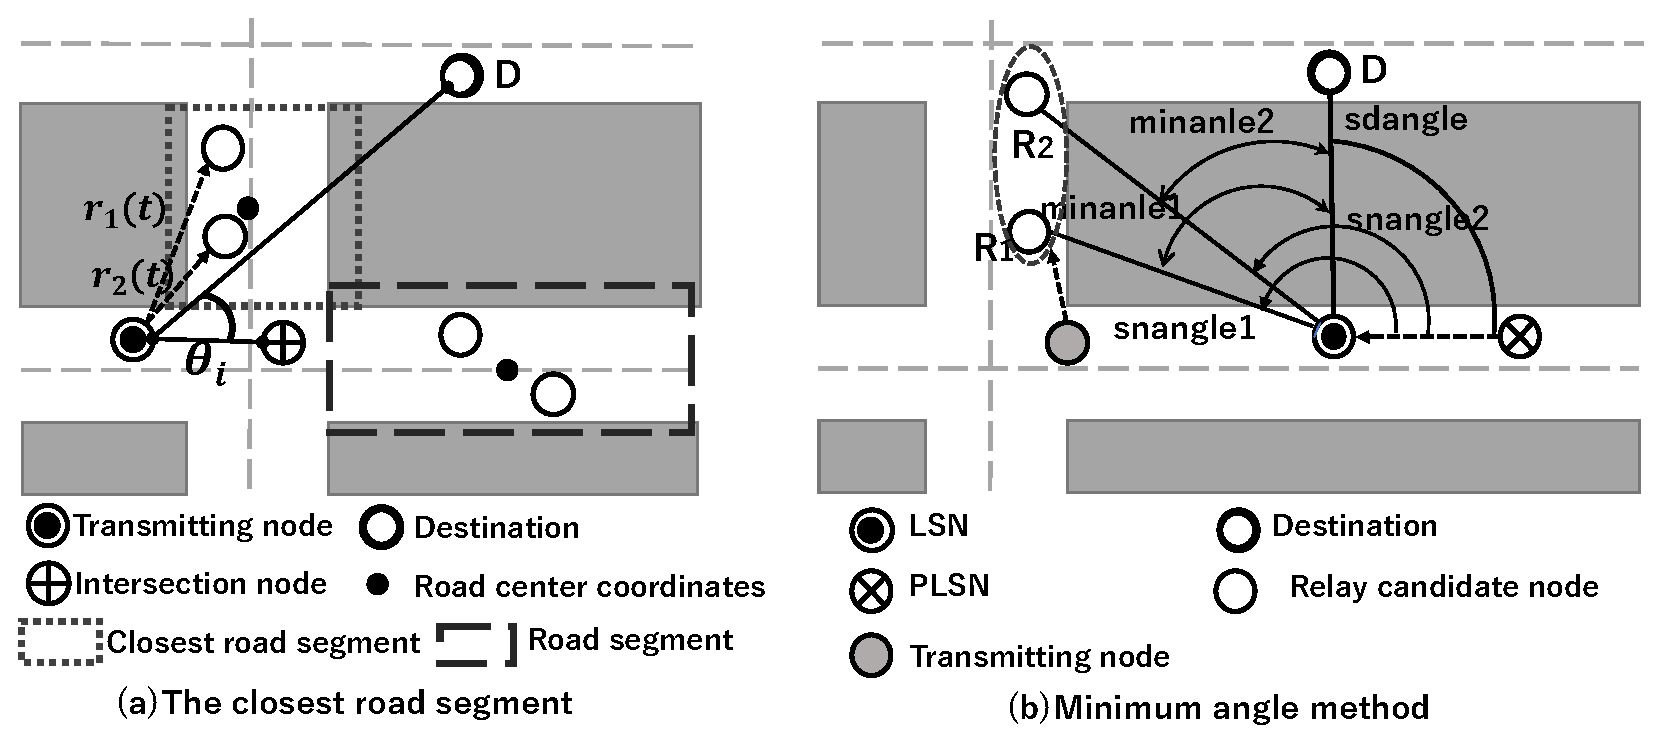
\includegraphics[width=120mm]{figures/minangle.eps}
\caption{closest road segment and minimum angle method }
\label{fig:minagnle}
\end{figure}

\subsection{Priority scheduling algorithm}
In SIGO, a timer-based priority scheduling algorithm is used. 
In this algorithm, the node with the highest priority rebroadcasts the data packet first. 
When other relay candidate nodes overhear packets from nodes with a higher priority, they discard their pending packets. Each relay candidate node rebroadcasts the packet only when it has not received any packet from the node with a higher priority than itself until its timer expires.
In SIGO, the priority of node $i$ is calculated by the following equations (\ref{pri-intersection}) and (\ref{pri}).


\begin{equation}
\label{pri-intersection}
Priority = \frac{D_{sd} - D_{id}}{ETX_{i}^{2}} + IRI,  D_{id} < D_{sd}
\end{equation}

\begin{equation}
\label{pri}
Priority = \frac{D_{sd} - D_{id}}{ETX_{i}^{2}} ,   D_{id} < D_{sd}
\end{equation}

$D_{sd}$ is the distance from the transmitting node to the destination node, and $D_{id}$ is the distance from the relay candidate node $i$ to the destination node. 
$ETX_i$ represents link quality. $ETX_i$ is calculated in the same way as LSGO. 
Equation (\ref{pri-intersection}) is applied when node $i$ is a street intersection node, and equation (\ref{pri}) is applied when node $i$ is located outside the intersection. 
The larger the value calculated by equation (\ref{pri-intersection}) or (\ref{pri}), the higher the priority is assigned to node $i$. 


\subsection{Opportunistic recovery strategy(ORS)}

A recovery strategy is necessary to solve the local optimum problem. Unlike the traditional unicast type recovery strategy, we propose a broadcast type recovery strategy, that is, opportunistic recovery strategy (ORS) that broadcasts packets toward the relay candidate nodes set. Similar to the operations of OR, in ORS, a relay candidate node with a higher priority rebroadcasts the receiving packet. 
In the proposed ORS, the priority is determined using the link quality and the minimum angle method proposed in JBR. 
The node that first finds the local optimum situation is called the LSN,
and the previous node of the LSN is called the PLSN, i.e., LSN received the packet directly from PLSN. The LSN adds its position information to the packet and rebroadcasts it. If the packet arrives at a node closer to the destination than the LSN, it reverts to the regular relay strategy. Since the ORS uses the minimum angle method described later, the position information of both the LSN and PLSN is always included in the packet until the recovery strategy is completed.






\textbf{Conditions for relay candidate nodes in ORS.} 
In ORS, only neighbor nodes that satisfy Condition \ref{potential nodes} are relay candidate nodes.

\begin{equation}
\label{potential nodes}
\left( nldis_i > cldis \right)   AND   \left( nldis_i > mndis_i \right) 
\end{equation}

where $cldis$ is the distance between the previous node(i.e., transmitting node received the packet directly from previous node) and transmitting node,
$nldis_i$ is the distance between the previous node and the node under consideration(relay candidate node $i$), and $mndis_i$ is the distance between the transmitting node and the relay candidate node $i$.


\textbf{minimum angle method.} Initially, as we can see in Fig \ref{fig:minagnle}(b), each transmitting node or LSN calculate $sdangle$. The angle between the lines connecting the LSN to the destination node and connecting the LSN and PLSN. The next step, each transmitting node or LSN calculate $snangle_i$. The angle between the lines connecting the LSN to the relay candidate node $i$  and connecting the LSN and PLSN. The last step is the calculation of  $minangle$ (Equation \ref{minangle}).

\begin{equation}
\label{minangle}
minangle_i = \mid sdangle - snangle_i \mid
\end{equation}


\textbf{ORS priority scheduling algorithm.} 
The priority of relay candidate node $i$ is calculated by the following equations \ref{sameORS} and \ref{diffORS}.


\begin{equation}
\label{sameORS}
Priority = \frac{360 - minangle_i}{ETX_{i}^{2}} + mndis
\end{equation}

\begin{equation}
\label{diffORS}
Priority = \frac{360 - minangle_i}{ETX_{i}^{2}} 
\end{equation}

Equation \ref{sameORS}  is applied when relay candidate node $i$ exists in the same road segment as the transmitting node or relay candidate node is intersection node. Otherwise, equation \ref{diffORS} is applied.



\section{Evaluation}

To evaluate the usefulness of the proposed OR, we compared it with the LSGO protocol for two evaluation metrics: packet delivery ratio (PDR) and overhead. 
The PDR is the ratio of the total number of packets received by the destination node to the total number of packets sent by the source node. The overhead is the total number of data packets transmitted by all nodes in the entire network divided by the total number of data packets successfully received by the destination nodes. 
In addition, we evaluated SIGO with JBR or ORS to investigate the usefulness of the proposed opportunistic recovery strategy. We used NS3\footnote{https://www.nsnam.org/} simulator, and the simulation parameters in Table \ref{tab:parameter}. Figure \ref{fig:evaluation}(a) shows the simulation scenario. 



\begin{table}[!ht]
\begin{center}
\caption{Simulation parameters}
\label{tab:parameter}
\begin{tabular}{|l|l|lll}
\cline{1-2}
Simulator    & NS-3 (v3.30)   &  &  &  \\ \cline{1-2}
Simulation area    & 1000m × 1000m   &  &  &  \\ \cline{1-2}
Number of vehicles & 400      &  &  &  \\ \cline{1-2}
Radio propagation model    & obstacle shadowing model\cite{obstacle}&  &  &  \\ \cline{1-2}
Number of relay candidate nodes  & 5       &  &  \\ \cline{1-2}
Shadowing parameter   & 10db ~ 30db      &  &  &  \\ \cline{1-2}
Weighting factor $\alpha$  & 1.0      &  &  &  \\ \cline{1-2}
\end{tabular}
\end{center}
\end{table}

\begin{figure}[!ht]
\centering
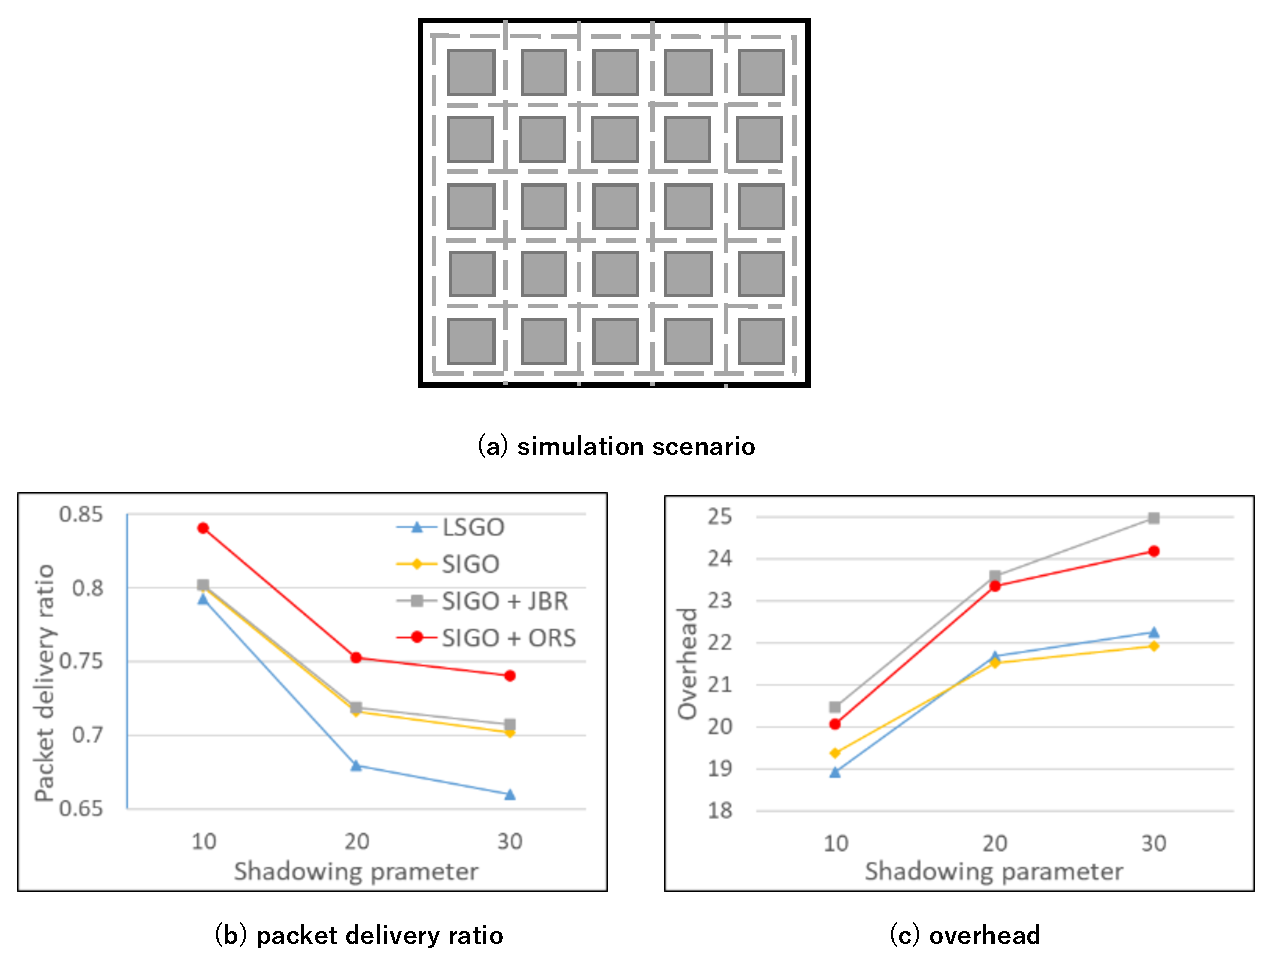
\includegraphics[width=120mm]{figures/evaluation.eps}
\caption{simulation scenario and PDR and overhead }
\label{fig:evaluation}
\end{figure}





We used the obstacle shadowing model\cite{obstacle} as the propagation model. The obstacle shadowing model has a shadowing parameter, i.e., the attenuation per meter(dB). 
Figure \ref{fig:evaluation}(b) and (c) show PDR and overhead, respectively.  As shown in these figures, the communication performance of SIGO is improved compared to LSGO as the shadowing parameter increases for both PDR and overhead. This is because SIGO does not increase the number of packets transmitted compared to LSGO, but forms a route that is less susceptible to shadowing, which increases the number of packets that reach the destination node. These figures also show the ORS has improved communication performance compared to JBR. The ORS improves PDR by 4 \% on average compared to JBR. JBR's recovery strategy uses one relay node (Unicast) and does not consider link quality. Therefore, JBR has hardly succeeded in recovery. 

 


\section{Conclusion}
We proposed new OR named SIGO and ORS. We also demonstrated them effectiveness in improving compared to existing scheme.



% \section*{Acknowledgments}

% Your acknowledgments to co-workers and financial sponsors are placed here.

\end{document}
